\chapter{Introduction}
\label{chapter:introduction}

%\minitoc
\chapterwithfigures{\nameref*{chapter:introduction}}
%\chapterwithtables{\nameref*{chapter:introduction}}

\ifthenelse{\boolean{skipIntro}}{\endinput}{}

\emph{Perspicere} - \textit{to see through}. The concept of perspective is rooted in the idea of projecting our three-dimensional world onto a two-dimensional plane. It has been studied for centuries, with its earliest fundation found in the geometry defined by Euclide in his \cite{euclide}. During the Quattrocento in the Italian Renaissance, Florence's artists and architects pioneered the study of linear perspective, striving to accurately represent the surrounding world. Brunelleschi (1377-1446) was among the first to study how lines, shapes, and objects change when observed from different viewpoints and angles. Linear perspective is characterized by lines of sights converging at one or more vanishing points and aims to replicate how objects appear to the human eye. Painting depicted on Figure \ref{fig:arnolfini} from Jan van Eyck is remarkable from a perspective standpoint: the chandelier, furniture and tiles are meticuloustly represented to align with the perspective. It demonstrates how linear perspective, with precise geometric proportions, can instantaneously create an illlusion of depth on a flat surface. 

\begin{figure}[htp!]
      \begin{center}
      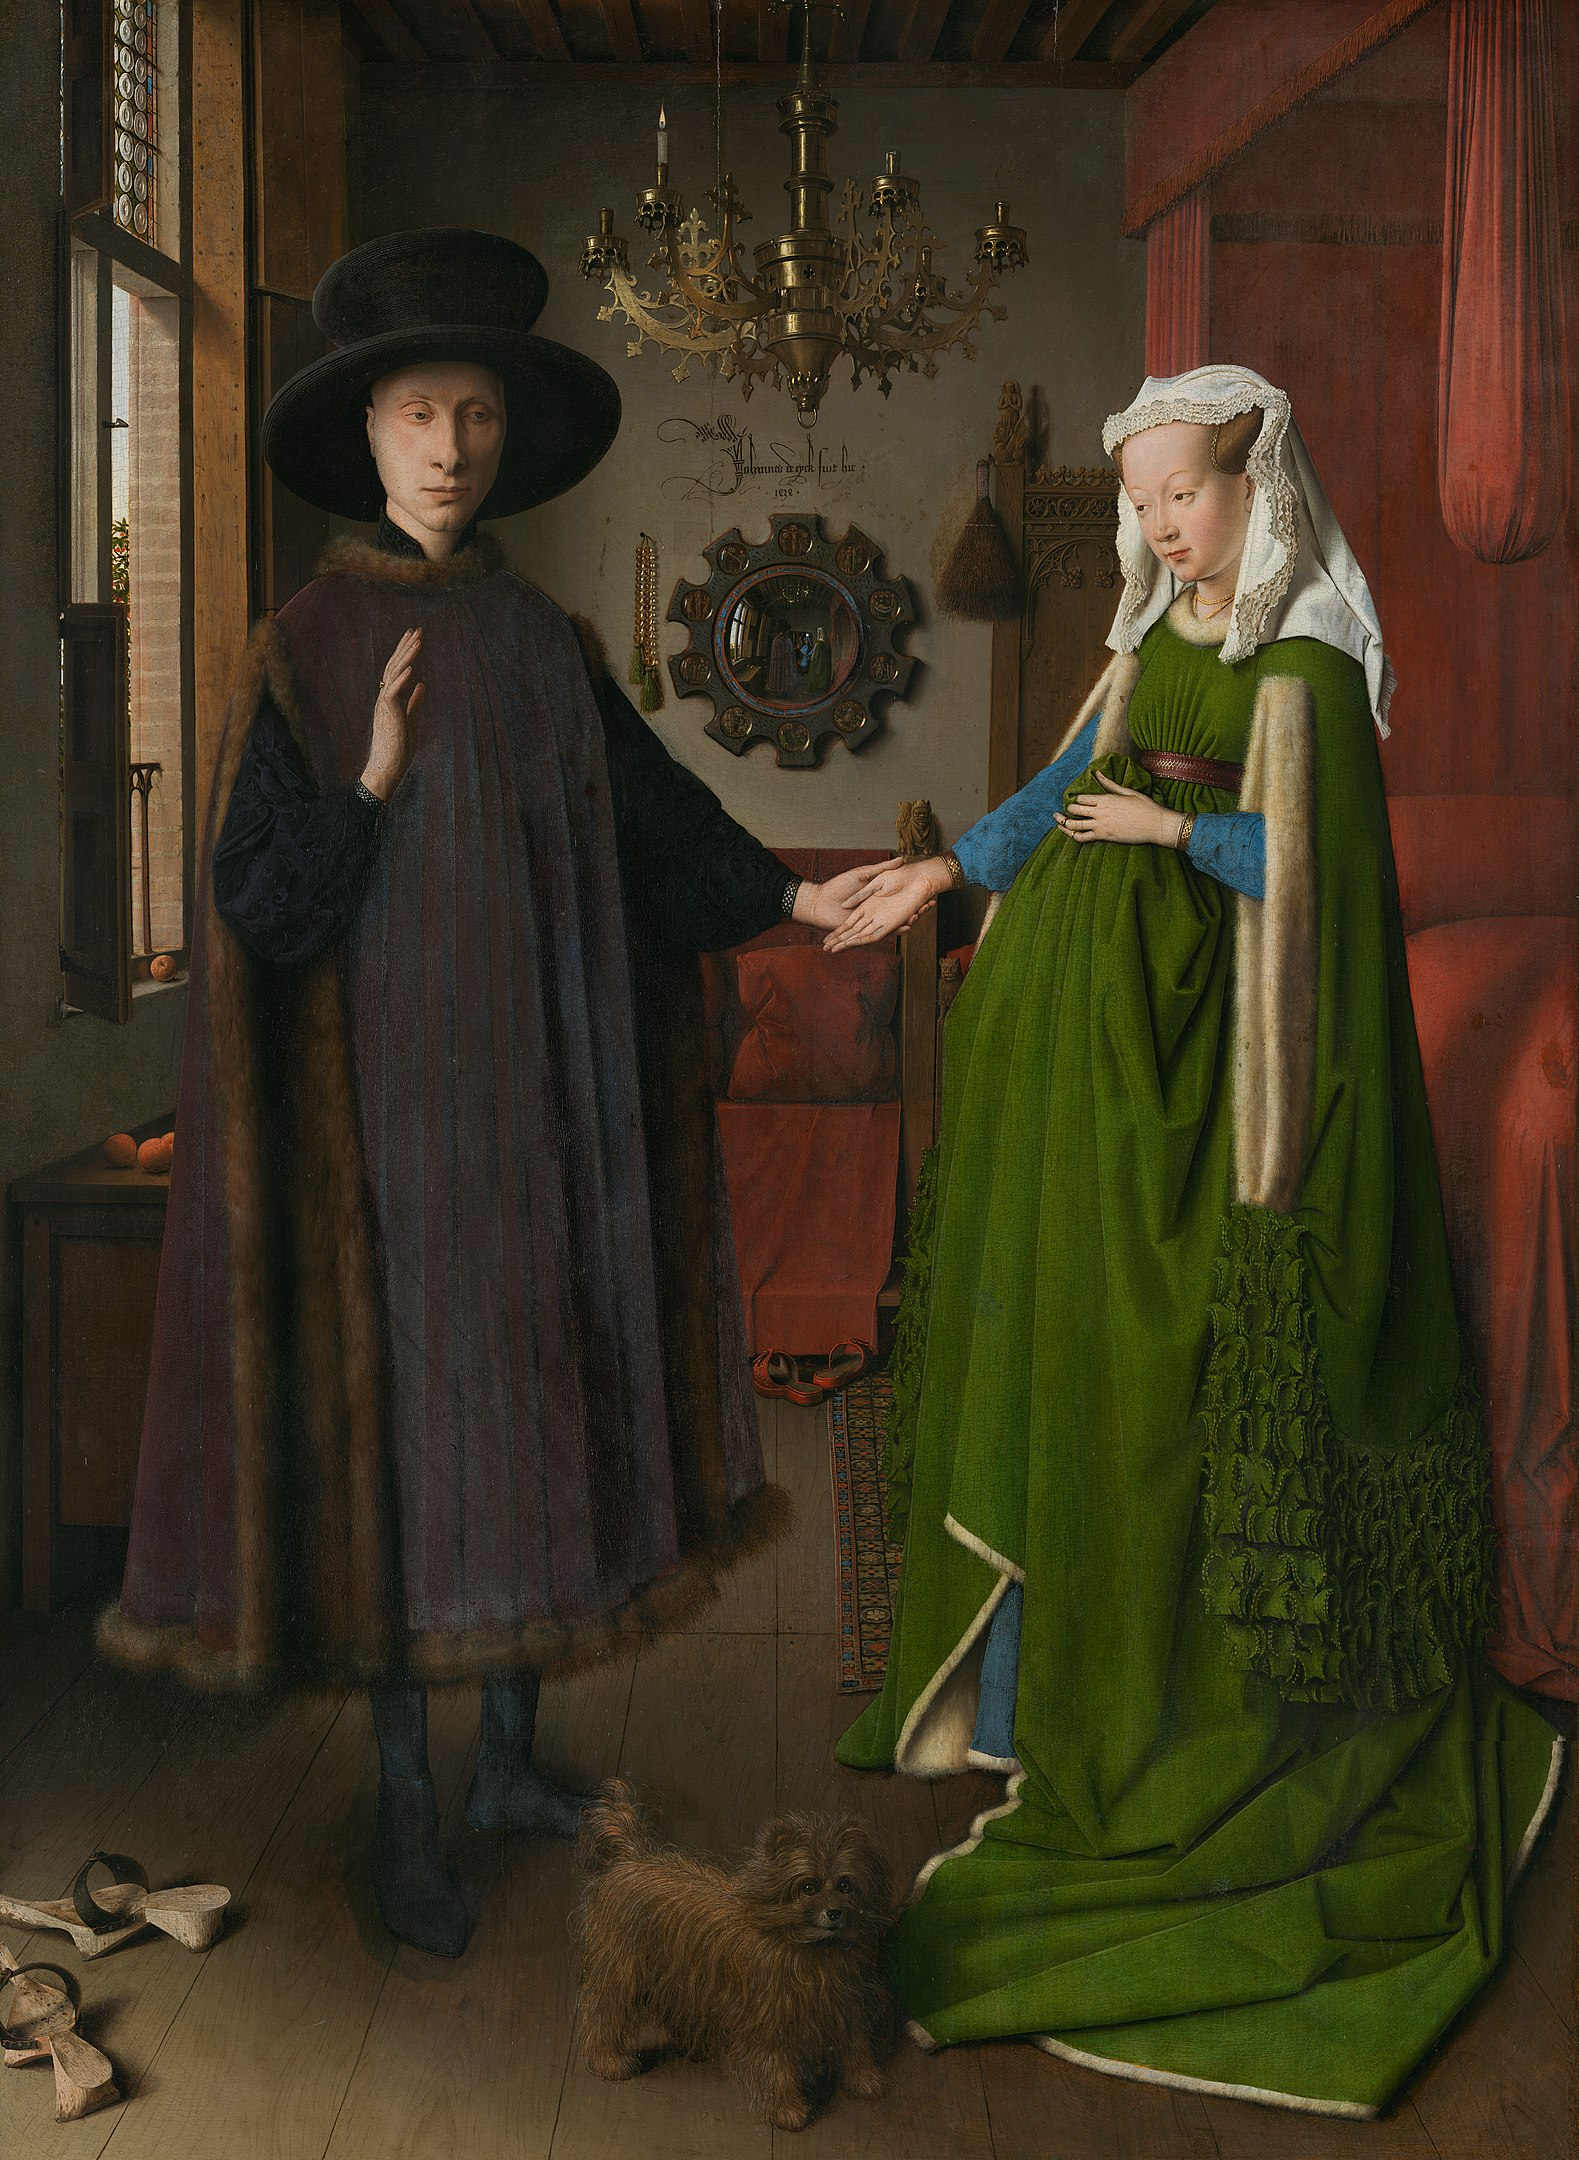
\includegraphics[width=\textwidth]{images/introduction/The_Arnolfini_portrait.jpg}
      \end{center}
      \caption{\textbf{\textit{The Arnolfini portrait},1434 - Jan van Eyck ($\sim$ 1390-1441)}. Such a 600 year old painting is renowned for its detailed realism and its innovative use of perspective.}
      \label{fig:arnolfini}
\end{figure}

Although artistic studies of perspective were highly refined from a technical and mechanical standpoint \citep{simon2021jan}, perspective found new applications in sciences a few centuries later with the development of photogrammetry. The term derives from its Greek etymology, \textit{photo} (\ie light), \textit{gramma} (\ie drawing or writing) and \textit{metron} (\ie measure). In 1849, Aimé Laussedat, a French astronomer, geodesist, surveyor and cartographer used the \textit{Hôtel des Invalides} to observe, measure and attempt to reproduce physical spaces, lines and objects from multiples perspectives. An illustration of a technical drawing he made for the Vincennes castle in 1850 is shown in Figure \ref{fig:intro_laussedat}. Photogrammetry leverages the parallax effect to extract depth and dimensions from the physical world based on observed views and was widely used in the mid last century for military purposes. The advent of aerial photography, enabled by advancements in aviation, allowed for the topographic mapping of entire countries during the interwar period.

\begin{figure}[htp!]
      \begin{center}
      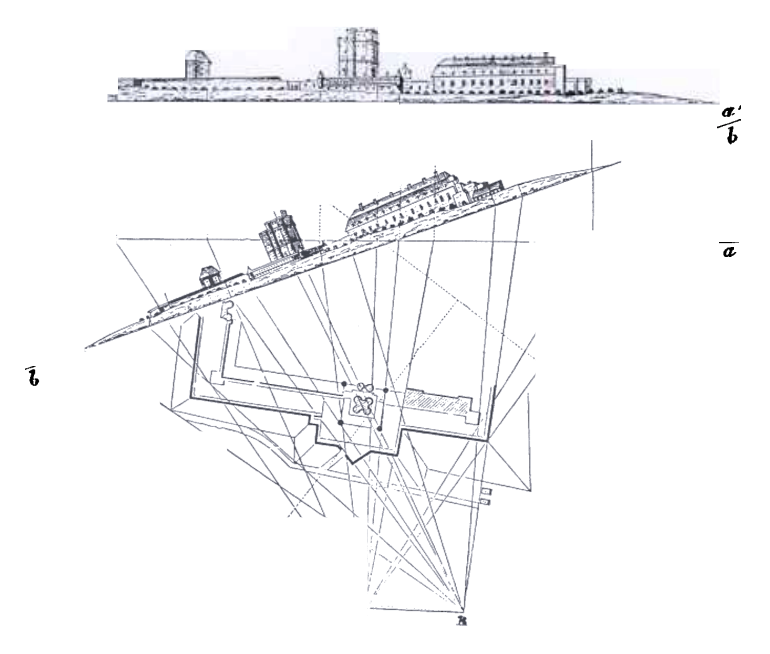
\includegraphics[width=.5\textwidth]{images/introduction/laussedat_phtograpmetrie.png}
      \end{center}
      \caption{\textbf{Survey of the Château de Vincennes by A. Laussedat, 1850.} Surveyed by the method of graphical intersections applied to perspectives recorded with the camera lucida. }
      \label{fig:intro_laussedat}
\end{figure}

Photogrammetry bacame a heavily studied field in the 1980's, notably in robotics and computer vision, thanks to increasing computational power and emerging digital imaging technologies. \ac{SfM} approaches naturally arised from the growing convergence between photogrammetry and computer vision during this period, pioneered by the work of Shimon Ullman \citep{ullman1979interpretation}. Such a domain paved the way for novel view synthesis issues and 3D reconstruction by bridging the gap between photographic scenes capturing processes and their three-dimensional representation. 

\ac{AI}, despite its broad, often unclear, and sometimes debated definition in society, has a long history spanning over 70 years. Alan Turning, widely regarded as one of the founding fathers of computer science \citep{turing1950computing}, and John McCarthy, a pionner in artificial intelligence, laid the foundations for the field. According to \href{https://www.britannica.com/technology/artificial-intelligence}{The Encyclopedia Britannica}, \ac{AI} is defined as \textit{"the ability of a computer to perform tasks commonly associated with intelligent beings"}. In the realm of computer vision and graphics, this manuscript focuses on a shrinked domain of \ac{AI}, commonly refered as \ac{DL}: \ac{DNN} and neural rendering are thus going to be considered in a large extend in the next few pages.

\ac{DL} has a fascinating and outstanding history. One of most influential figures in vision community is Yann LeCun. Over the past 30 years, he has made significant contributions to vision \ac{AI}, and notably introduced \ac{CNN} \citep{lecun1998gradient}. These \ac{NN} have played a key role in the research that were conducted during the last three year of this thesis. The release of ImageNet \citep{deng2009imagenet} in 2009, a million annotated images database, along with the \ac{CNN}-based image classifier AlexNet \citep{krizhevsky2012imagenet} in 2012, is unanimously seen as the breakthrough moment for \ac{DL}. Vision tasks tackled by these \ac{DL} algorithms have grown in complexity, from segmentation \citep{long2015fully} to detection \citep{girshick2015fast}, and even image generation model such as \ac{GAN} \citep{goodfellow2014generative}. While image-based vision tasks have seen substantial profress over the last decade, only recently has the third dimension, addressing 3D issues in the physical world, been seriously considered, driven by the latest advances in \ac{GPU} computing. The most recent \ac{DL} architectures are now capable of generating high-quality, textured 3D mesh from a single image. An output produced by InstantMesh \citep{xu2024instantmesh}, one of the latest state-of-the-art single-image 3D reconstruction method, is shown in Figure \ref{fig:intro-instantmesh}. This thesis positions itself within the emerging field of 3D \ac{AI}, which is poised for significant growth in the coming years, focusing on the integration of 3D geometric priors for \ac{NVS}.  


\begin{figure}[htp!]
      \centering
      \begin{subfigure}{0.48\linewidth}
        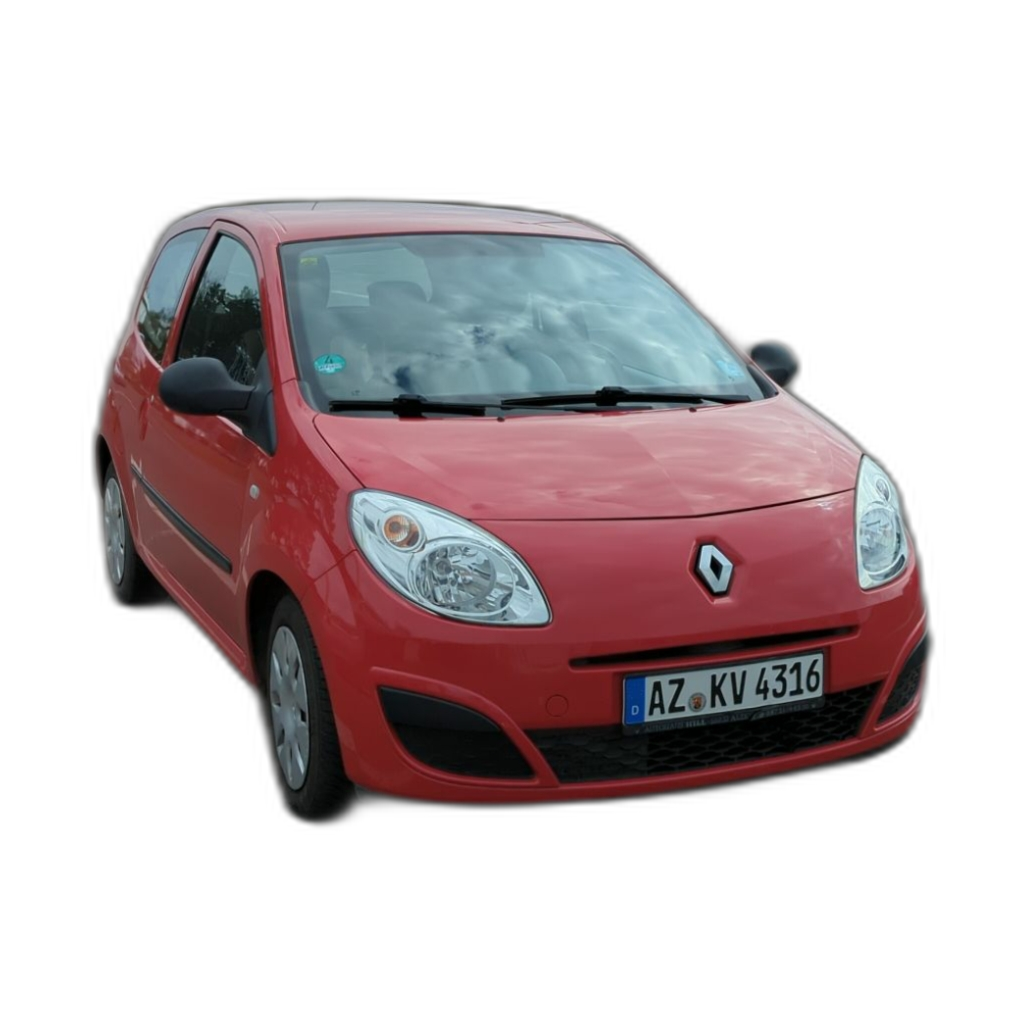
\includegraphics[width=.7\linewidth]{images/introduction/input-instantmesh.png}
        \caption{Input image}
      \end{subfigure}
      \hfill
      \begin{subfigure}{0.48\linewidth}
        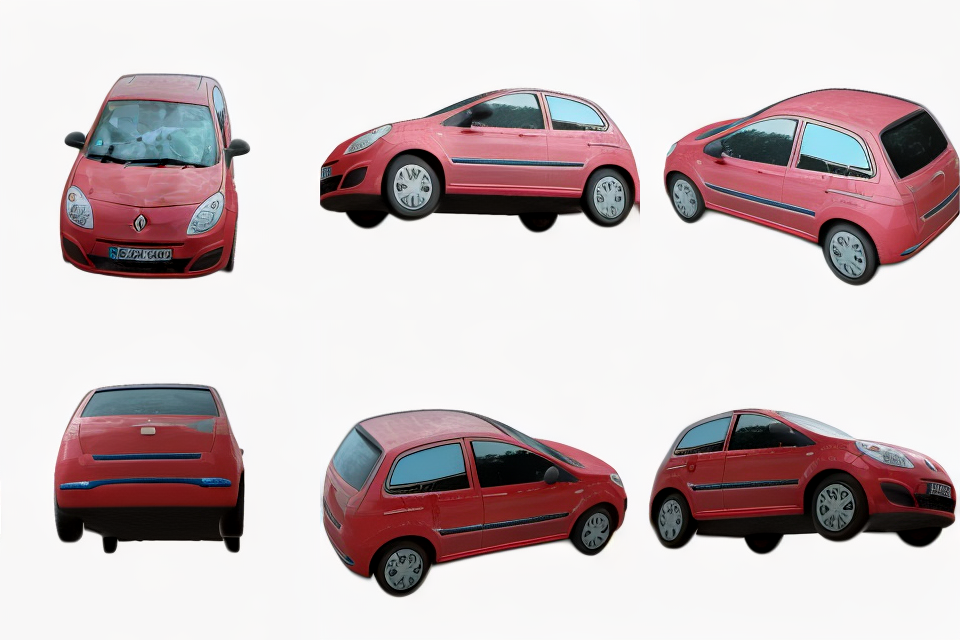
\includegraphics[width=\linewidth]{images/introduction/output-instantmesh.png}
        \caption{Novel views}
      \end{subfigure}
      \caption{\textbf{InstantMesh rendered views from generated 3D mesh.} (a) InstantMesh takes as input a single image of an unique object set on a white background. (b) Novel views from the car can be obtained by rendering the produced 3D mesh.}
    \label{fig:intro-instantmesh}
    \end{figure}

\section{PhD Context}

\subsection{Meero}
Meero is a French \ac{SaaS} startup founded in 2014 that primarily provides \ac{AI}-powered visual enhancement tools and algorithms for businesses in various sectors, including real estate agencies, e-commerce and fashion industries, as well as automotive car dealerships. Meero offers a wide range of \ac{AI}-based solutions, from sky replacement, virtual staging or object removal algorithms for the real-estate industry, as well as background removal and virtual try-on for fashion and e-commerce companies. In its automotive branch, branded as \textit{CarCutter}, Meero brings car dealerships and marketplaces tools to produce visually consistent and appealing images. One of its latest products, the 360\degree spin, enables users to produce stabilized and coherent views of a car given a limited set of images. This 3D-based application is in a large extent presented in the last chapter of this thesis.

However, fundamental research and industrial applications in computer vision suffers from a massive gap that needs to be closed. Most academic papers in vision research focus on images ranging in size from $128\times128$ to $1024\times1024$ pixels, while images from any mobile device now have resolution of at least 2K (up to 4 to 6K for the latest \ac{DSLR} cameras). Although this gap is narrowing thanks to the latest fundation models and rapidly advancing \ac{GPU} compute capabilities, this discrepancy in image resolution remains a challenge. It prevents direct translation of image-based \ac{AI} product from academic research to industy. This thesis aims to address this gap, primarily by investigating generalizable single-image \ac{NVS} architectures that are not restricted to a single scene. 

\subsection{3D reconstruction}
 \ac{NVS} is inherently intertwined with 3D reconstruction, as the synthesis of novel views became feasible once a complete 3D representation was acquired. A variety of approaches exists to address this issue; ranging from photogrammetry-based or Structure-From-X techniques (where X could stands for \textit{Motion} \citep{longuet1981computer}, \textit{Shading} \citep{horn1989obtaining} or \textit{Silhouette} \citep{baumgart1974geometric} for instance) to structured-lights ones. Pionnering work in this area includes considerations of stereo vision \citep{marr1976cooperative} through an iterative cooperative algorithm between two views. 
 
The first \ac{AI}-based 3D reconstruction algorithms began to emerge in 2018, with seminal research by \citep{kato2018neural} introducing one of the first differentiable neural renderer within a \ac{DL} pipeline. The release of PyTorch3D \citep{ravi2020pytorch3d} in 2020 for \ac{DL}-based 3D code development significantly constributed to the widespread adoption of 3D techniques within the scientific community. Recent groundbreaking advances in 2023 and 2024, from multi-view \citep{li2023neuralangelo} to single-image \citep{voleti2024sv3d} 3D reconstruction, herald an exciting future for research in this field.

3D reconstruction and \ac{NVS} meets each other in this thesis through the \autoref{chapter:gausssplat}, where a 3D scene must first to be explicitly reconstructed before rendering novel viewpoints from unseen locations. 

\subsection{Novel View Synthesis}
\ac{NVS} is a challenging task in computer vision, wherein the objective is to generate an image from an unobserved viewpoint using only a limited number of source images and their corresponding camera pose information. This thesis focuses on the most difficult scenario, which relies exclusively on a unique source image. In 1998, Thomas Vetter introduced an innovative approach \citep{vetter1998synthesis} for single face image \ac{NVS}, where multiple views were used to \textit{learn} pose-invariant descriptors by leveraging a generic 3D model of the human head. Since 2015, \ac{NVS} has increasingly been explored through the \ac{AI} prism \citep{yang2015weakly}, even though camera displacements were first discretized, preventing novel views to be rendered from any random viewpoints. The field benefited in late 2020 with the introduction of a simple yet outstandingly powerful framework known as \ac{NeRF} \citep{mildenhall2020nerf}. A year ago, 3D\ac{GS} models have once again disrupted the field by enabling real-time novel view synthesis with 2K  images on a consumer \ac{GPU}. 


\section{Contributions}
\ac{NVS} from a single image has several plausible solutions and is therefore considered as an ill-posed problem. There are too many details, structures or texture that remain unobserved with a single source view. The core issue arising from this observation is the need to find ways, such as efficient pose encoding or structural constraints, that can provide as much prior information as possible to the \ac{NN}. 

Prior to the emergence of foundation models \citep{awais2023foundational} and \ac{GenAI}\footnote{We make a clear distinction with the first generative networks that were build in 2014 on \ac{GAN} \citep{goodfellow2014generative} considerations}, dataset images used in single-image \ac{NVS} were mostly low resolution ones, usually $128\times128$ as in ShapeNet \citep{chang2015shapenet}. Throughout this thesis, we aimed to incorporate epipolar geometric constraints to the greatest extent possible. We remain convinced by a guiding principle that has shaped our work over the past three years: \textit{the most fundamental 3D geometric considerations, such as epipolar geometry, must be explicitly integrated into deep neural networks.}

We tackle the \ac{NVS} problem with several approaches during this thesis, that could be summarized as follow.
\begin{itemize}
      \item \autoref{chapter:epipolarnvs}: \nameref{chapter:epipolarnvs}\\
            We begin our single-image \ac{NVS} exploration through the prism of camera transformation encoding. This information is essential for any \ac{NN} that performs \ac{NVS}, and integrating it as prior information is not a trivial task. While several approaches exist to give intrinsic and extrinsic parameters to a network, we introduce a novel method in this chapter that extensively leverages on epipolar geometry to encode camera transformations. The work in this chapter has led to the following conference publication:
            \begin{itemize}
                \item \fullcite{landreau2022epipolarnvs}
            \end{itemize}

      \item \autoref{chapter:epinerf}: \nameref{chapter:epinerf}\\
            We then shift our focus from camera pose encoding to the consideration of internal 3D constraints within \ac{NeRF} architectures. However, we retain the concept of epipolar geometry in our work and develop a feature-based attention mechanism through an additional \ac{NeRF}-based network, called \textit{NeRFeature}. This mecanism is direclty involved at training time, while we \textit{do not} have access to the target view for building epipolar constraints. Our work is currently under review at 3DV:
            \begin{itemize}
                  \item \fullcite{landreau2024epinerf}
            \end{itemize}

      \item \autoref{chapter:gausssplat}: \nameref{chapter:gausssplat}\\
            We relaxed the primary hypothesis addressed in the first two apparoches to deal on \ac{NVS} with a multi-images scenario with 3D\ac{GS}. Such a work primarily relates to the industrial challenges posed by \textit{CarCutter} around the next generation of the current 360\degree spin stabilization. While rendering at training locations is successful from a quality perspective, stabilizing the camera path to render unobserved viewpoint is crutial for creating seamless 360\degree car animations. 

      \item \autoref{chapter:appendix-adaptativeSR}: \nameref{chapter:appendix-adaptativeSR} \\
      The first tree contributions were extensively focused on \ac{NVS}. This fourth and final work is more closely related to 3D reconstruction issues but remains connected to the original problem this thesis addresses. It examines topological considerations for 3D meshes produced by a single-image 3D reconstruction \ac{NN}. We designed a module called \textit{AdaptativeSR}, which prunes mesh faces by accounting only 2D rendered silhouette masks. The work in this annex has led to the following conference publication:
      \begin{itemize}
            \item \fullcite{landreau2022adaptativesr}
      \end{itemize}
\end{itemize}


